\documentclass[border=10pt,tikz,multi]{standalone}
\usetikzlibrary{angles,shadows.blur,positioning,backgrounds}
\usepackage[dvipsnames]{xcolor}
\usepackage{amsmath}
\usepackage{amssymb}

\begin{document}
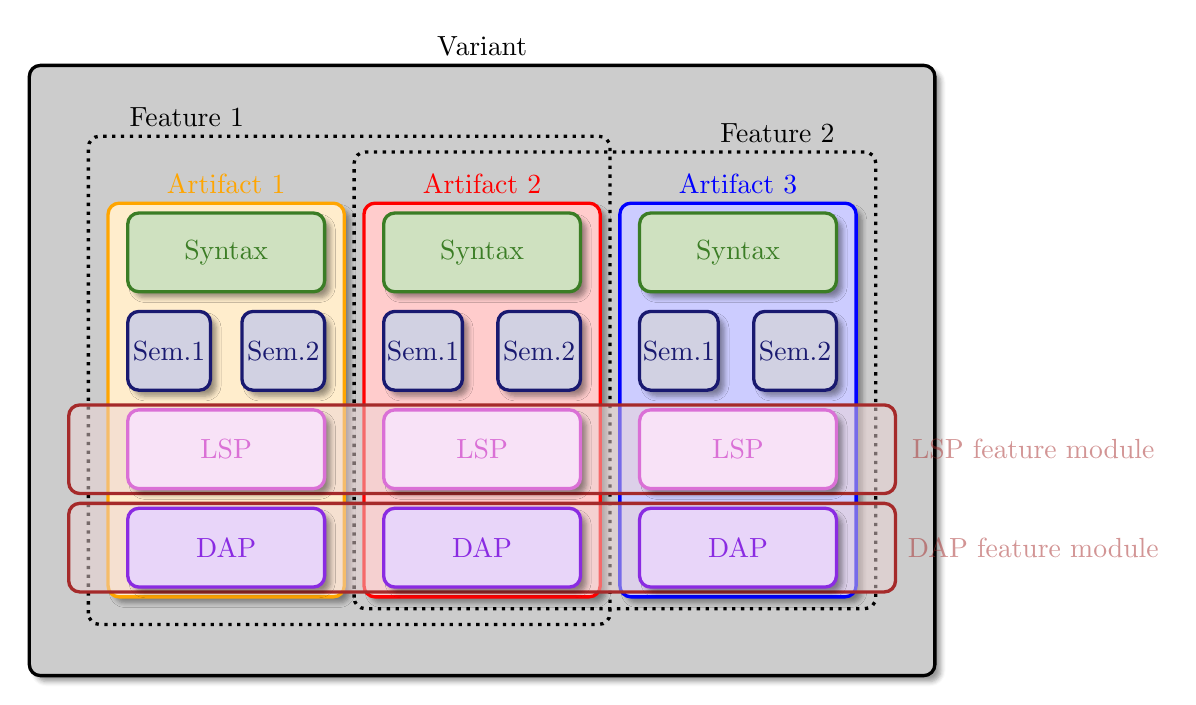
\begin{tikzpicture}
% dashed,
    % \draw[dashed, very thick, rounded corners, anchor=north]
    %         (3.75,-0.25) rectangle (8.25,3.75)
    %         node[anchor=north, align=center] at (6.125,4.25) {$\mathcal{L} + \mathcal{E}$};

% ============================
\draw[Black, very thick, rounded corners, anchor=north, fill=Black!20, blur shadow={shadow blur steps=5}]
        (-1, -1) rectangle (10.5, 6.75)
        node[anchor=north, align=center] at (4.75,7.25) {Variant};

% ============================
\draw[dotted, very thick, rounded corners, anchor=north]
        (-0.25,-0.35) rectangle (6.375, 5.85)
        node[anchor=north, align=center] at (1,6.35) {Feature 1};

\draw[dotted, very thick, rounded corners, anchor=north]
        (3.125,-0.15) rectangle (9.75, 5.65)
        node[anchor=north, align=center] at (8.5,6.15) {Feature 2};

% ============================

\draw[Orange, very thick, rounded corners, anchor=north, fill=Orange!20, blur shadow={shadow blur steps=5}]
        (0,0) rectangle (3, 5)
        node[anchor=north, align=center] at (1.5,5.5) {Artifact 1};

\draw[Red, very thick, rounded corners, fill=Red!20, blur shadow={shadow blur steps=5}]
    (3.25,0) rectangle (6.25,5)
    node[anchor=north, align=center] at (4.75,5.5) {Artifact 2};

\draw[Blue, very thick, rounded corners, fill=Blue!20, blur shadow={shadow blur steps=5}]
    (6.5,0) rectangle (9.5,5)
    node[anchor=north, align=center] at (8,5.5) {Artifact 3};

% ============================
\draw[Brown, very thick, rounded corners, fill=Brown!20, fill opacity=0.5]
        (-0.5,0.0625) rectangle (10, 1.1875)
        node[] at (11.75,0.625) {DAP feature module};

\draw[Brown, very thick, rounded corners, fill=Brown!20, fill opacity=0.5]
        (-0.5,1.3125) rectangle (10, 2.4375)
        node[] at (11.75,1.875) {LSP feature module};

% ============================

\draw[OliveGreen, very thick, rounded corners, fill=OliveGreen!20, blur shadow={shadow blur steps=5}]
    (0.25,3.875) rectangle (2.75,4.875)
    node[pos=.5] {Syntax};

\draw[MidnightBlue, very thick, rounded corners, fill=MidnightBlue!20, blur shadow={shadow blur steps=5}]
    (0.25,2.625) rectangle (1.3,3.625)
    node[pos=.5] {Sem.1};

\draw[MidnightBlue, very thick, rounded corners, fill=MidnightBlue!20, blur shadow={shadow blur steps=5}]
    (1.7,2.625) rectangle (2.75,3.625)
    node[pos=.5] {Sem.2};

\draw[Orchid, very thick, rounded corners, fill=Orchid!20, blur shadow={shadow blur steps=5}]
    (0.25,1.375) rectangle (2.75,2.375)
    node[pos=.5] {LSP};

\draw[BlueViolet, very thick, rounded corners, fill=BlueViolet!20, blur shadow={shadow blur steps=5}]
    (0.25,0.125) rectangle (2.75,1.125)
    node[pos=.5] {DAP};

% ============================

\draw[OliveGreen, very thick, rounded corners, fill=OliveGreen!20, blur shadow={shadow blur steps=5}]
    (3.5,3.875) rectangle (6,4.875)
    node[pos=.5] {Syntax};

\draw[MidnightBlue, very thick, rounded corners, fill=MidnightBlue!20, blur shadow={shadow blur steps=5}]
    (3.5,2.625) rectangle (4.5,3.625)
    node[pos=.5] {Sem.1};

\draw[MidnightBlue, very thick, rounded corners, fill=MidnightBlue!20, blur shadow={shadow blur steps=5}]
    (4.95,2.625) rectangle (6,3.625)
    node[pos=.5] {Sem.2};

\draw[Orchid, very thick, rounded corners, fill=Orchid!20, blur shadow={shadow blur steps=5}]
    (3.5,1.375) rectangle (6,2.375)
    node[pos=.5] {LSP};

\draw[BlueViolet, very thick, rounded corners, fill=BlueViolet!20, blur shadow={shadow blur steps=5}]
    (3.5,0.125) rectangle (6,1.125)
    node[pos=.5] {DAP};

% ============================

\draw[OliveGreen, very thick, rounded corners, fill=OliveGreen!20, blur shadow={shadow blur steps=5}]
    (6.75,3.875) rectangle (9.25,4.875)
    node[pos=.5] {Syntax};

\draw[MidnightBlue, very thick, rounded corners, fill=MidnightBlue!20, blur shadow={shadow blur steps=5}]
    (6.75,2.625) rectangle (7.75,3.625)
    node[pos=.5] {Sem.1};

\draw[MidnightBlue, very thick, rounded corners, fill=MidnightBlue!20, blur shadow={shadow blur steps=5}]
    (8.2,2.625) rectangle (9.25,3.625)
    node[pos=.5] {Sem.2};

\draw[Orchid, very thick, rounded corners, fill=Orchid!20, blur shadow={shadow blur steps=5}]
    (6.75,1.375) rectangle (9.25,2.375)
    node[pos=.5] {LSP};

\draw[BlueViolet, very thick, rounded corners, fill=BlueViolet!20, blur shadow={shadow blur steps=5}]
    (6.75,0.125) rectangle (9.25,1.125)
    node[pos=.5] {DAP};

% ============================


\end{tikzpicture}

\end{document}
